\section{Introduction}\label{s:intro}

Its somewhat hard to properly explain the depth of the rabbit hole I have fallen into with my thesis research. It started out somewhat simple, I had this very basic idea in mind, what if you took a part of a program, and rewrote it in different programming languages and kind of like legos slotted it into place of the original program. Now this isn't by any means a new idea, I honestly just had a mild curiosity in how that would work given that I've never really wrote and executed some distinct program which was written in two different languages. In a way that idea felt somewhat odd, especially if you consider languages with completely different execution methods; how do languages even communicate with one another. 

So to begin this `little' exploration I had to first thing of a piece of software I could use to actually test this idea with. Before doing so I thought it would be important to maybe further define my idea beyond just wanting to test out my "lego theory". As said before the concept of rewriting code is by no means new, I don't believe it would be absurd by any means to suggest that most programmers at one point or another, while writing some piece of code, or even after the fact, recognized ways in which their solution can be improved. Often times improvements or iterations on the original piece of code just naturally have to occur to fit the evolving goal for a given piece of software. There are countless examples of this but going into this but we should get back to the matter at hand. So we can say that there should be some type of reason as to why we want to rewrite a specific piece of code, in our case performance would be a pretty natural choice. While most programming languages of course aim to be performant due to differences in their design and execution methods they naturally exhibit differences. 

Ok, so we want to choose a piece of software, preferably one with a performance critical component, which we want to rewrite. Looking back at my previous projects one specifically came to mind, my implementation of a simple Ray Tracer in the Julia programming languages based on Peter Shirley's wonderful guide and C++ implementation. My initial goal with this project was to learn Julia using a *totally-reasonably-sized-project* as I had heard and seen that if written in a very idiomatic manner it can exhibit performance characteristics close of that to C while offering the dynamically typed simplicity of Python. Naturally when benchmarking my final implementation my results where less then desirable. To elaborate on why my program exhibited these performance characteristics it makes sense briefly go into the core of how Julia code is actually run. There is a very nice quote I found on the Julia forums a while back which I believe effectively conveys this

\begin{quote}
    \textit{in short, it's a reasonably good static compiler but a terrible JIT}
\end{quote}

The first response some people might have to this is confusion. Julia is a JIT compiled languages so how is its JIT terrible. Well this comes down in large part to how its JIT works, the core of this is how it preforms online partial evaluation (OPE) w.r.t. its type system. OPE w.r.t the type system in this instance refers to the process of, at runtime (online), Julia specializes (partially evaluates) methods for which it can infer the types of every local variable from the types of the arguments or any other constants; in this instance a method is said to be "type stable". Specializing type stable methods simply means it compiles methods for the set of concrete types it can infer. Practically speaking this mechanism can also be seen as a form of **monomorphizing** a set of functions for which the JIT compiler can determine the concrete types. The reason then why Julia's JIT compiler could be called "terrible" would be that it, currently at least, does not implement profile guided optimization (PGO). The lack of PGO and its reliance on type stable code for speed means that there is a causation between idiomatically written Julia and its performance. With this understanding it might now be apparent why my Ray-Tracer preformed so poorly, as I was not fully aware of this strong dependence and I simply wrote the code how I would write something in any other dynamically typed high-level language.

We've now established that we have a piece of performance critical software written in a very non-idiomatic and by extension inefficient manner. Furthermore we've seen that its execution method is not only different from ahead of time (AOT) compiled languages but also from other JIT compiled languages by its unique approach to generating machine code. The conventional route, and quite frankly recommended route, one should go here would be to simply rewrite everything with Julia's idiomatic principles in mind, though this would lead to a rather short and likely failing thesis, so question the alternative, what if we rewrote the most performance critical segment of our ray tracer in a language which has less reliance on a unique idiomatic programming style. While at first this seems somewhat nonsensical it has the potential to raise and in turn answer some interesting questions about interoperability and more generally code execution methods including but not limited to:
\begin{itemize}
    \item How do we design a system of communication between languages which exhibit considerable fundamental differences?
    \item How do we reconcile different type systems in language interoperability?
    \item What are the performance characteristics of language interoperability?
\end{itemize}

% \TODO{
% This section includes the context and motivation behind the work, explicitly or implicitly highlights the main research question(s), provides a high-level explanation of the solution, and describes the contributions.}

% \TODO{Context, motivation, research question asds, and original contribution could be organized in subsections.}

% Rewriting software components; or entire systems; in a different language is a common practice to address various limitations caused by the original implementation language, including but not limited to performance, maintainability, and scalability. The primary motivation behind rewriting is to leverage the strengths of the new language to address the limitations of the original language. However, rewriting a large system, especially in a different language with potentially different paradigms can be a complex and time-consuming task. This study aims to asses the viability of leveraging language interoperability to simplify and expedite the rewriting process.
% Most well known major software services today like Facebook, YouTube, Google, LinkedIn, Wordpress, etc. have all had either components many of them starting out with language such as PHP or Ruby on Rails because these were the popular choices back in the day and what the intial developers where likely the most familiar with. We can take YouTube as a good example, it was intially written largely in PHP, but as the platform grew this came with some key drawbacks, a key one being scalability, one reason for switching to Python (and C++) was because Python speifically had both a wider range of syntax expressions and more importantly a better optimizability. This allowed for rapid flexible development and deployment, in addition to scalability and performance at an improved maintainability over PHP.\  
% Similar stories exist for so many other platforms, as languages evolve and the second system effect comes into play we will naturally see software evolve to adapt to new requirements and technologies as developers realize their mistakes of the past. Though the rewriting process does not come without its own set of challenges. It could be argued that a contributing factor to the downfall of the Netscape browser was the decision to do a ground up rewrite of the browser, a reason for this being that the original code base was so messy developers did not want to contribute \textcite{pogue2000netscape}. The choice was then made to start from new, but by the time the browser released it still lacked a lot of basic features \textcite{zawinski1999resignation}. 
% More broadly speaking the manner in which we choose to rewrite software in a different language should preferably align with the core motivation as best as we can, while mitigating as many of the downsides as possible. This is where the concept of language interoperability could come into play. Language interoperability can potentially offer some very interesting benefits, a key one being the ability to effectively implement a gradual/iterative rewrite while still allowing for the original code to be used. The benefit here being that we can leverage the strengths of the new language, still use existing familiar infrastructure, all while allowing the system to be iteratively improved without there being any major downtime untill the rewrite is complete.

% ---------- templates for figures ----------------------- 

% \begin{figure}[bh]
%     %% The macro `\onecolgrid' is defined in `vusec.sty'
%     %% NOTE: The suffix "./figures/" is implicitly included for this relative path.
%     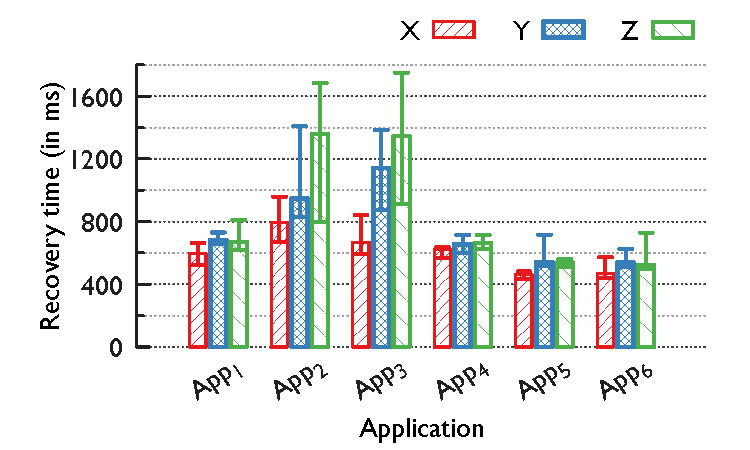
\includegraphics[width=\onecolgrid]{cache-by-app}
%     %% Labels should immediately follow caption, to keep latex quiet.
%     \figcap{Simple one-column figure. Please include a brief explanation or takeaway.}\label{fig:1col}
% \end{figure}

% \begin{figure*}[th]
%     %% The macro `\threecolgrid' is defined in `vusec.sty'
%     \begin{subfigure}[t]{\threecolgrid}
%         %% NOTE: The suffix "./figures/" is implicitly included for these relative paths.
%         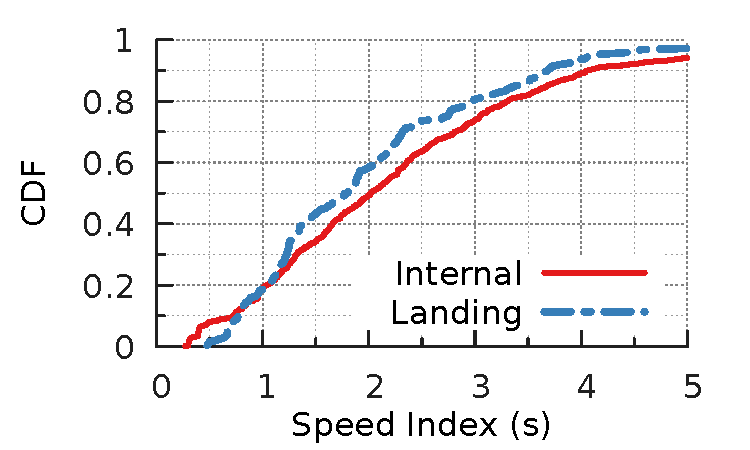
\includegraphics[width=\linewidth]{three-col/speed_index}
%         \sfigcap{}\label{fig:3col-a}
%     \end{subfigure}
%     \begin{subfigure}[t]{\threecolgrid}
%         %% NOTE: You do not have to mention the extension.
%         %% (The example figures are in PDF format.)
%         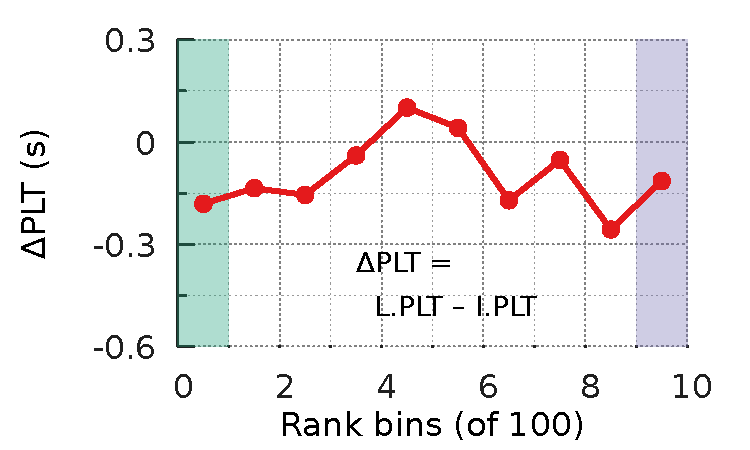
\includegraphics[width=\linewidth]{three-col/plt_ranks_diff}
%         \sfigcap{}\label{fig:3col-b}
%     \end{subfigure}
%     \begin{subfigure}[t]{\threecolgrid}
%         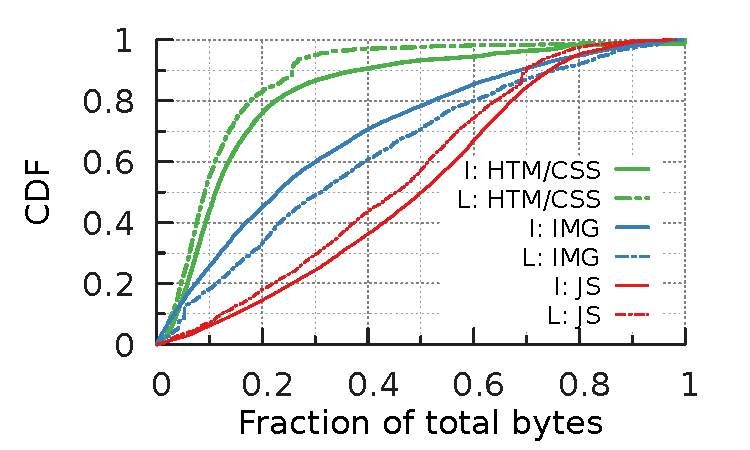
\includegraphics[width=\linewidth]{three-col/mimes}
%         \sfigcap{}\label{fig:3col-c}
%     \end{subfigure}
%     %% Labels should immediately follow caption, to keep latex quiet.
%     \figcap{Generate clear and beautiful figures (in PDF) that can be rendered side by side while still being easy to read and interpret. Choose colors wisely from the colorbrewer2.org website.}\label{fig:3col}
% \end{figure*}

% \begin{table}[hb]
%     \centering
%     \tabcap{A simple table describing the characteristics of a data set or the results of an experiment}\label{tab:sample}
%     \taburulecolor{black!45}
%     \begin{tabu}{c|c|r|r|r|r}
%         \toprule
%         \multirow{2}{*}{\thead{Char.}} &
%             \multirow{2}{*}{\thead{\#samples}} &
%             \thead{Count} &
%             \multicolumn{3}{c}{\thead{Perf. Score}}\\
%         &
%             &
%             \thead{of items} &
%             \thead{X} & \thead{Y} & \thead{Z} \\
%         \midrule
%         \stress{P}
%             & 214 & 56 & 9 & 23 & 24 \\
%         \stress{Q}
%             & 117 & 27 & 7 & 10 & 10 \\
%         \stress{R}
%             & 222 & 11 & 6 & 4 & 1 \\
%         \stress{S}
%             & 187 &  9 & 1 & 6 & 2 \\
%         \stress{T}
%             & 180 & 16 & 7 & 5 & 4 \\
%         \bottomrule
%     \end{tabu}

% \end{table}

 